    \begin{tikzpicture}[node distance=2cm,scale=0.6,every node/.style={transform shape}]

      \record(
      0,
      \small{\texttt{a:Person}},
      \small{\texttt{name:Tolkien}},
      $\boldsymbol{\rightarrow}$ \textbf{\small{\texttt{wrote b}}},
      \texttt{edge},
      \texttt{edge}
      );

      \record(
      -1,
      \small{\texttt{b:Book}},
      \texttt{property},
      \small{\texttt{title:The \hspace{-0.15cm} Hobbit}},
      ,
      \texttt{edge}
      );

      \record(-2,
      \small{\texttt{vertex id}},
      \texttt{property},
      \texttt{property},
      \texttt{edge},
      \texttt{edge}
      );


      \spaceRecord(-3)

      \record(-4,
      \small{\texttt{vertex id}},
      \texttt{property},
      \texttt{edge},
      \texttt{edge},
      \texttt{edge}
      );

    \end{tikzpicture}
